%% AMS-LaTeX Created with the Wolfram Language for Students - Personal Use Only : www.wolfram.com

\documentclass{article}
\usepackage{amsmath, amssymb, graphics, setspace}

\newcommand{\mathsym}[1]{{}}
\newcommand{\unicode}[1]{{}}

\begin{document}

\title{Benard Cell analysis}
\author{}
\date{}
\maketitle

\section*{Schema}

A simple Benard cell can be represented by three parts: the heater \(H\), the cooler \(C\) much bigger than the system of interest \(S\) which is
placed in between the two. The analysis usually goes along this lines: if the temperature difference between the heater and the cooler \(\text{$\Delta
$T}=T_H-T_C\) is small then the heat transfer occurs by diffusion, however if the temperature difference a critical point a second mechanism, convection,
engages in heat transfer.

\(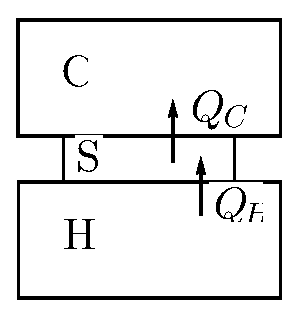
\includegraphics{Benard Cell_gr1.eps}

\)

Benard cell schema; the heater and cooler are in thermal equilibrium.

\section*{Analysis}

We{'}ll analyze it from the perspective of internal entropy produced (\(i\)) and external entropy transferred \((e)\) to the system of interest \(S\).
Of course entropy change of the system \(dS_S\) would be the sum of those two:

\(\frac{dS_S}{dt}=\frac{dS_i}{dt}+\frac{dS_e}{dt}\)

In our analysis we{'}ll limit ourselves to the scenario of a stable state in which the same amount of heat that goes in also goes out. In other words
\(Q_C=-Q_H\) and we get

\(dS_e=\frac{dQ_H}{T_H}+\frac{dQ_C}{T_C}=dQ_H\left(\frac{1}{T_H}-\frac{1}{T_C}\right)=dQ_H\left(\frac{T_C-T_H}{T_HT_C}\right)<0\)

Therefore the process transfers some of the entropy outside the system. However, since we require a stable state \(dS_S=0\) it leads us to the conclusion
that \(dS_i=-dS_e>0\), so in a sense we could say that the rate of internal entropy production \(dS_i\) is a function of the entropy inflow \(dS_e\).
Moreover the entropy gets lowered by negative inflow of entropy, so \(S-S_0<0\), where \(S_0=S(t=0)\).

If we now consider a scenario in which \(j_e=\frac{dS_e}{dt}\) was non$--$zero for some time and then turned off, then by Tylor expansion

\(\frac{dS_i}{dt}=j_i(S)=j_i\left(S_0\right)+\left(S-S_0\right)C_1+\mathcal{O}\left(S^2\right)\)

and noticing that \(j_i\left(S_0\right)=0\) by definition (if the inflow of entropy is null, then the system stays in equilibrium) and therefore
\(C_1\) has to be negative since \(j_i(S)>0\) and \(S-S_0<0\).\\
Further we rewrite the equation with \(C_1=-\frac{1}{\tau }\) (\(\tau\) positive)

\(\frac{dS_i}{dt}=j_i\left(S_i\right)=\frac{S_0-S_i}{\tau }+\mathcal{O}\left(S^2\right)\)

and solve this equation:

\begin{doublespace}
\noindent\(\pmb{\text{DSolve}\left[y'[t]\text{==}\frac{\text{y0}-y[t]}{\tau },y[t],t\right]}\)
\end{doublespace}

\begin{doublespace}
\noindent\(\left\{\left\{y[t]\to \text{y0}+e^{-\frac{t}{\tau }} C[1]\right\}\right\}\)
\end{doublespace}

\(S_i(t)=S_0\left(1-e^{-t/\tau }\right)+S_1e^{-t/\tau }\)

\begin{doublespace}
\noindent\(\pmb{\text{Plot}\left[\left\{2,3e^{-\frac{t}{\tau }} +2\left(1-e^{-\frac{t}{\tau }}\right),4e^{-\frac{t}{\tau }} +2\left(1-e^{-\frac{t}{\tau
}}\right),1e^{-\frac{t}{\tau }} +2\left(1-e^{-\frac{t}{\tau }}\right) \right\}\text{/.}\{\tau \text{-$>$}1\},\right.}\\
\pmb{\{t,0,5\},\text{PlotLabels}\to \left\{S_0\right\},\text{AxesLabel}\to \left\{\text{t},\texttt{"}S_i\text{(t)$\texttt{"}$}\right\},\text{Ticks}\to
\text{None},}\\
\pmb{\text{PlotRange}\to \text{Full}]}\)
\end{doublespace}

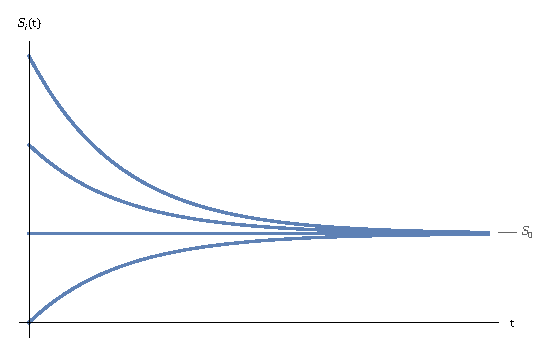
\includegraphics{Benard Cell_gr2.eps}

Therefore the system returns to equilibrium as expected

However if consider an equation in which \(j_e\neq 0\) then we get a different solution

\begin{doublespace}
\noindent\(\pmb{\text{DSolve}\left[y'[t]==\text{je}+\frac{\text{y0}-y[t]}{\tau },y[t],t\right]}\)
\end{doublespace}

\begin{doublespace}
\noindent\(\left\{\left\{y[t]\to \text{y0}+\text{je} \tau +e^{-\frac{t}{\tau }} C[1]\right\}\right\}\)
\end{doublespace}

\(S_i(t)=S_0+j_e\tau \left(1-e^{-t/\tau }\right)\)

The entropy smoothly lowers to minimum entropy

\begin{doublespace}
\noindent\(\pmb{\text{Plot}\left[\left\{\text{y0}+\text{je} \tau +e^{-\frac{t}{\tau }} \text{/.}\{\tau \to 1,\text{y0}\to 2,\text{je}\to 1\},3\right\},\{t,0,5\},\text{PlotRange}\to
\{\{0,5\},\{2.7,4\}\},\right.}\\
\pmb{\left.\text{PlotLabels}\to \left\{S_i[t],S_{\min }\right\},\text{AxesLabel}\to \left\{\text{t},\texttt{"}S_i\text{(t)$\texttt{"}$}\right\},\text{Ticks}\to
\text{None}\right]}\)
\end{doublespace}

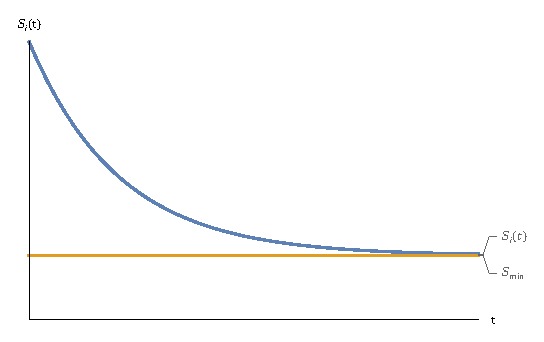
\includegraphics{Benard Cell_gr3.eps}

and we see that \(j_i\to j_{\max }=\frac{S_0-S_{\min }}{\tau }=-j_e\). 

The Benard cell doesn{'}t store energy, hence internal energy stays constant, but since as we saw entropy get{'}s minimized at steady state that
means that free energy, defined by

\(F=U-T\, S\)

gets maximized. This free energy again allows us to perform work which in this case is visualized in the circular, convective motions of the fluid.

Now we may make a weak association with information $--$ since erase of information is associated with entropy production (due to Landauer), then
we can say that at steady$--$state the amount of information stays constant, even though the it{'}s inflow is non$--$zero (negative \(dS_e\)) it
get{'}s immediately erased by the non$--$zero internal entropy production (positive \(dS_i\))

[Calculation of complexity]

Problem jaki widz$\unicode{0119}$, to to, $\unicode{017c}$e te r{\' o}wnania s$\unicode{0105}$ spe{\l}nione r{\' o}wnania s$\unicode{0105}$ spe{\l}nione
r{\' o}wnie$\unicode{017c}$ podczas dyfuzji, a wi$\unicode{0119}$c nie m{\' o}wi$\unicode{0105}$ nam nic specjalnego o konwekcji i dlatego cz{\l}on
\(\left.dS_i\right/dt\) nie mo$\unicode{017c}$e by{\' c} uto$\unicode{017c}$samiony z MEP (kt{\' o}ry nie wyst$\unicode{0119}$puje np. blisko stanu
r{\' o}wnowagi)

\end{document}
